\noindent
\begin{minipage}[t]{0.48\textwidth}
  \noindent (c)\enspace Bạn nên lái xe ở tốc độ nào nếu muốn tiết kiệm xăng nhất?

  \vspace{0.3em}
  \begin{center}
    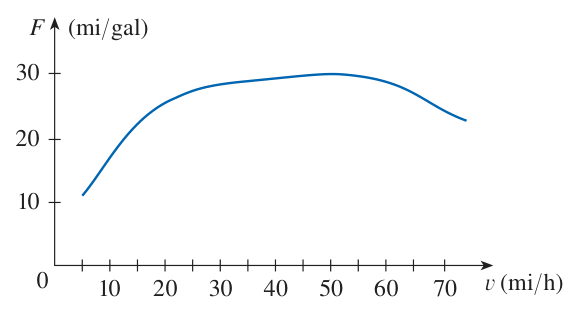
\includegraphics[width=0.88\linewidth]{images/p0198_fig1.png}
  \end{center}
  \vspace{0.2em}

  \textbf{15.}\enspace Đồ thị cho thấy nhiệt độ trung bình của nước bề mặt $f$ của hồ Michigan biến thiên như thế nào trong suốt một năm (trong đó $t$ được đo bằng tháng với $t = 0$ tương ứng với ngày 1 tháng 1). Giá trị trung bình được tính toán từ các số liệu thu thập trong khoảng thời gian 20 năm kết thúc vào năm 2011. Hãy vẽ phác thảo đồ thị của hàm đạo hàm $f'$. Khi nào thì $f'(t)$ đạt giá trị lớn nhất?

  \vspace{0.3em}
  \begin{center}
    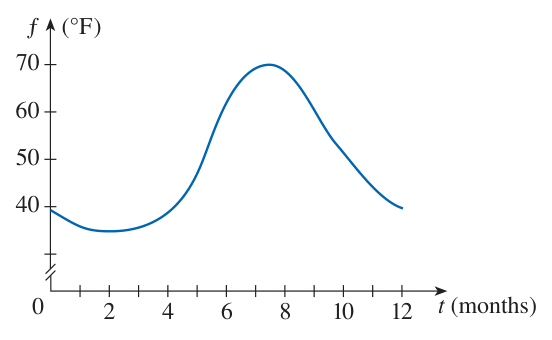
\includegraphics[width=0.88\linewidth]{images/p0198_fig2.png}
  \end{center}
  \vspace{0.2em}

  \noindent\textbf{\color{stewartcyan}16--18}\enspace Hãy vẽ cẩn thận đồ thị của $f$ và ở ngay phía dưới hãy vẽ phác thảo đồ thị của $f'$ theo cách tương tự như trong các Bài tập 4--11. Bạn có thể đoán một công thức cho $f'(x)$ từ đồ thị của nó không?

  \vspace{0.4em}
  \noindent
  \textbf{16.}\enspace $f(x) = \sin x$\hfill
  \textbf{17.}\enspace $f(x) = e^x$\hfill
  \textbf{18.}\enspace $f(x) = \ln x$

  \vspace{0.5em}
  \noindent{\color{stewartrule}\rule{\linewidth}{0.6pt}}
  \vspace{0.4em}

  \noindent\llap{\casicon\hspace{4pt}}\textbf{19.}\enspace Cho $f(x) = x^2$.
  \begin{enumerate}[label=(\alph*), leftmargin=*, topsep=2pt, itemsep=1.5pt]
    \item Ước tính các giá trị của $f'(0)$, $f'(\frac{1}{2})$, $f'(1)$, và $f'(2)$ bằng cách phóng to đồ thị của $f$.
    \item Sử dụng tính đối xứng để suy ra các giá trị của $f'(-\frac{1}{2})$, $f'(-1)$, và $f'(-2)$.
    \item Sử dụng các kết quả từ các phần (a) và (b) để đoán một công thức cho $f'(x)$.
    \item Sử dụng định nghĩa của đạo hàm để chứng minh rằng phán đoán của bạn ở phần (c) là đúng.
  \end{enumerate}

  \vspace{0.3em}
  \noindent\llap{\casicon\hspace{4pt}}\textbf{20.}\enspace Cho $f(x) = x^3$.
  \begin{enumerate}[label=(\alph*), leftmargin=*, topsep=2pt, itemsep=1.5pt]
    \item Ước tính các giá trị của $f'(0)$, $f'(\frac{1}{2})$, $f'(1)$, $f'(2)$, và $f'(3)$ bằng cách phóng to đồ thị của $f$.
    \item Sử dụng tính đối xứng để suy ra các giá trị của $f'(-\frac{1}{2})$, $f'(-1)$, $f'(-2)$, và $f'(-3)$.
    \item Sử dụng các giá trị từ các phần (a) và (b) để vẽ đồ thị của $f'$.
    \item Đoán một công thức cho $f'(x)$.
    \item Sử dụng định nghĩa của đạo hàm để chứng minh rằng phán đoán của bạn ở phần (d) là đúng.
  \end{enumerate}
\end{minipage}%
\hfill
\begin{minipage}[t]{0.48\textwidth}
  \noindent\textbf{\color{stewartcyan}21--32}\enspace Tìm đạo hàm của hàm số bằng cách sử dụng định nghĩa của đạo hàm. Nêu rõ tập xác định của hàm số và tập xác định của đạo hàm của nó.

  \vspace{0.4em}
  \noindent
  \begin{tabular}{@{}p{0.49\linewidth}@{\hspace{0.02\linewidth}}p{0.49\linewidth}@{}}
    \textbf{21.}\enspace $f(x) = 3x - 8$ & \textbf{22.}\enspace $f(x) = mx + b$ \\[6pt]
    \textbf{23.}\enspace $f(t) = 2.5t^2 + 6t$ & \textbf{24.}\enspace $f(x) = 4 + 8x - 5x^2$ \\[6pt]
    \textbf{25.}\enspace $A(p) = 4p^3 + 3p$ & \textbf{26.}\enspace $F(t) = t^3 - 5t + 1$ \\[8pt]
    \textbf{27.}\enspace $f(x) = \dfrac{1}{x^2 - 4}$ & \textbf{28.}\enspace $F(v) = \dfrac{v}{v + 2}$ \\[14pt]
    \textbf{29.}\enspace $g(u) = \dfrac{u + 1}{4u - 1}$ & \textbf{30.}\enspace $f(x) = x^4$ \\[14pt]
    \textbf{31.}\enspace $f(x) = \dfrac{1}{\sqrt{1 + x}}$ & \textbf{32.}\enspace $g(x) = \dfrac{1}{1 + \sqrt{x}}$
  \end{tabular}

  \vspace{0.7em}
  \noindent{\color{stewartrule}\rule{\linewidth}{0.6pt}}
  \vspace{0.4em}

  \noindent\textbf{33.}\enspace (a) Vẽ phác thảo đồ thị của $f(x) = 1 + \sqrt{x + 3}$ bằng cách bắt đầu từ đồ thị của $y = \sqrt{x}$ và sử dụng các phép biến đổi đồ thị ở Mục 1.3.
  \begin{enumerate}[label=(\alph*), leftmargin=*, topsep=2pt, itemsep=1.5pt]
    \setcounter{enumi}{1}
    \item Sử dụng đồ thị ở phần (a) để vẽ phác thảo đồ thị của $f'$.
    \item Sử dụng định nghĩa của đạo hàm để tìm $f'(x)$. Tập xác định của $f$ và $f'$ là gì?
    \item[\llap{\casicon\hspace{4pt}}(d)] Vẽ đồ thị của $f'$ và so sánh với hình phác thảo của bạn ở phần (b).
  \end{enumerate}

  \vspace{0.3em}
  \noindent\llap{\casicon\hspace{4pt}}\textbf{34.}\enspace (a) Nếu $f(x) = x + 1/x$, hãy tìm $f'(x)$.
  \begin{enumerate}[label=(\alph*), leftmargin=*, topsep=1pt, itemsep=1.5pt]
    \setcounter{enumi}{1}
    \item Kiểm tra xem câu trả lời của bạn ở phần (a) có hợp lý hay không bằng cách so sánh đồ thị của $f$ và $f'$.
  \end{enumerate}

  \vspace{0.3em}
  \noindent\llap{\casicon\hspace{4pt}}\textbf{35.}\enspace (a) Nếu $f(x) = x^4 + 2x$, hãy tìm $f'(x)$.
  \begin{enumerate}[label=(\alph*), leftmargin=*, topsep=1pt, itemsep=1.5pt]
    \setcounter{enumi}{1}
    \item Kiểm tra xem câu trả lời của bạn ở phần (a) có hợp lý hay không bằng cách so sánh đồ thị của $f$ và $f'$.
  \end{enumerate}

  \vspace{0.3em}
  \noindent\textbf{36.}\enspace Bảng số liệu cho biết số lượng $N(t)$, tính theo nghìn, các thủ thuật phẫu thuật thẩm mỹ xâm lấn tối thiểu được thực hiện tại Hoa Kỳ trong các năm $t$ khác nhau.

  \vspace{0.3em}
  \begin{center}
    \renewcommand{\arraystretch}{1.15}
    \begin{tabular}{|c|c|}
      \hline
      \rowcolor{stewarttablehead} \hspace{1.5em}$t$\hspace{1.5em} & \hspace{1em}$N(t)$ (nghìn)\hspace{1em} \\
      \hline
      2000 & 5.500 \\
      2002 & 4.897 \\
      2004 & 7.470 \\
      2006 & 9.138 \\
      2008 & 10.897 \\
      2010 & 11.561 \\
      2012 & 13.035 \\
      2014 & 13.945 \\
      \hline
    \end{tabular}
  \end{center}
  \vspace{-0.3em}
  \centerline{\fontsize{7.5pt}{9pt}\selectfont\textit{Nguồn: American Society of Plastic Surgeons}}
  \vspace{0.3em}

  \begin{enumerate}[label=(\alph*), leftmargin=*, topsep=1pt, itemsep=1.5pt]
    \item Ý nghĩa của $N'(t)$ là gì? Đơn vị của nó là gì?
    \item Hãy lập bảng các giá trị ước tính cho $N'(t)$.
    \item Vẽ đồ thị của $N$ và $N'$.
    \item Làm thế nào để có thể nhận được các giá trị chính xác hơn cho $N'(t)$?
  \end{enumerate}
\end{minipage}
